\pagestyle{fancy}
\normalsize
\linespread{1.5}\selectfont
\chapter{绪论}
\addtocontents{los}{\protect\addvspace{10pt}}

\section{研究背景}
领域特定语言的研究及应用日益广泛,其中不乏正则表达式、SQL、XML等应用场合及其多的领域特定语言。而随着计算机科学技术的发展,DSL的应用场景步入了日常生活中(引用IFTTT、IOS快捷指令)。而在一般场合中,语言设计者是计算机科学家,语言使用者却是领域内的专家。因此,当领域特定语言的使用出现一些问题时,领域内的专家(使用者)需要得到领域特定的信息来进行处理。

语法糖是近些年一种流行的领域特定语言实现方法,其方法源于Lisp的宏系统(Macro),经过Scheme语言的发展,再到Racket语言的扩展\upcite{frommacro}。语法糖构造DSL的最主要优点就是简单高效,语言设计者只需要写一个简单的映射,就可以构造DSL。

然而,语法糖的一项缺陷,导致其应用领域大多局限于计算机科学内部。我们先来看下面这个例子。

	我们拟构造一个自动化饭店的DSL\ref{fig:restaurant}为例。箭头表示语法糖展开的形式。
	
	\begin{figure}[h]
		\centering
		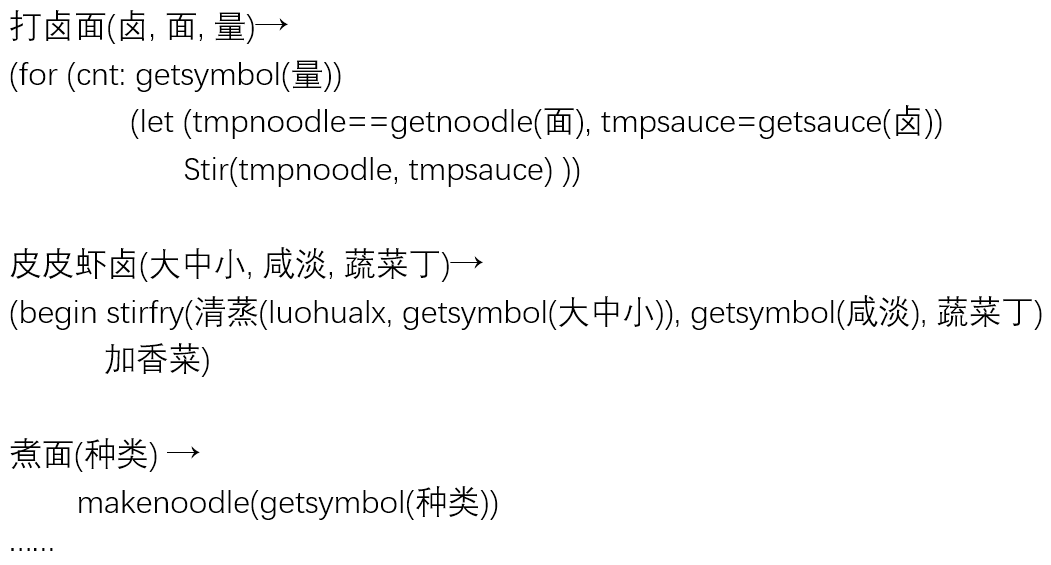
\includegraphics[width=12cm]{images/chapter1/restaurant.png}
		\caption{自动化饭店DSL}
		\label{fig:restaurant}
	\end{figure}

在这个DSL内,执行

\begin{flushleft}
	打卤面(皮皮虾卤(大,~ 咸,~ 胡萝卜),~ 煮面(毛细),~ 2)
\end{flushleft}

因为其过程中会有很多中间过程,我们期望得到的执行过程是这样的\ref{fig:expect}。
\begin{figure}[h]
	\begin{center}
		\framebox[35em][l]{
			\parbox[t]{\textwidth}{
				\begin{center}
					打卤面(皮皮虾卤(大,~ 咸,~ 胡萝卜),~ 煮面(毛细),~ 2)\\
					↓\\
					打卤面(皮皮虾卤(大,~ 咸,~ 胡萝卜丁),~ 煮面(毛细),~ 2)\\
					↓\\
					打卤面(大份咸皮皮虾卤(胡萝卜丁),~ 煮面(毛细),~ 2)\\
					↓\\
					打卤面(大份咸皮皮虾卤(胡萝卜丁),~ 毛细抻面,~ 2)\\
					↓\\
					两份皮皮虾打卤面(大份、咸、胡萝卜丁、毛细)
				\end{center}
				
			}
		}
	\end{center}
	\caption{期待的执行序列}
	\label{fig:expect}
\end{figure}


而实际上,这个DSL的执行序列是这样的\ref{fig:fact}。(先将语法糖展开成难懂的内部语言)
\begin{figure}[h]
	\begin{center}
		\framebox[35em][l]{
			\parbox[t]{\textwidth}{
				\begin{center}
					打卤面(皮皮虾卤(大,~ 咸,~ 胡萝卜),~ 煮面(毛细),~ 2)\\
					↓\\
					(begin~for$\ldots$~let($\ldots$)~$\ldots$)\\
					↓\\
					$\ldots$\\
					↓\\
					两份皮皮虾打卤面(大份、咸、胡萝卜丁、毛细)
				\end{center}
				
			}
		}
	\end{center}
	\caption{实际执行序列}
	\label{fig:fact}
\end{figure}


将这个例子抽象到简单的例子
	$and(or(\#f,~\#t),~and(\#t,~\#f))$

(其中and、or是语法糖,展开成if的表达式)有如下执行序列\ref{fig:desugar}

\begin{figure}[h]
	\framebox[35em][l]{
		\parbox[t]{\textwidth}{
			\begin{center}  
				and(or(\#f,~\#t),~and(\#t,~\#f))\\
				↓\\
				if(if(\#f,\#t, \#t), \#t, if(\#f, \#t, \#f))\\
				↓\\
				if(\#t , if(\#f, \#t, \#f), \#f)\\
				↓\\
				if(\#f, \#t, \#f)\\
				↓\\
				\#f
			\end{center}  
		}
	}  
\caption{语法糖表达式执行示例}
\label{fig:desugar}
\end{figure}

我们可以看到,在执行过程中,语法糖被展开成通用语言表达式,在通用语言中继续执行,得到最终结果。但实际应用到特定领域时,我们很明显不希望得到这样复杂的执行过程,特别是对于对计算机内部语言不熟悉的领域专家来说,这种执行过程是没有意义的。


\section{语法糖的困境}
\label{mark:onedirect}我们将上述问题总结为语法糖解糖的单向性,对上面的例子\ref{fig:desugar}的第三行

\begin{flushleft}
	$if(\#t , if(\#f, \#t, \#f), \#f)$
\end{flushleft}
进行观察,我们可以看出,其存在等价的领域特定语言表示$and(\#t, and(\#t, \#f))$,这正是初始表达式第一个子表达式规约后的结果。如果语法糖的解糖有一个逆过程(重组糖),我们就可以找到语法糖表达式其对应的在语法糖层面的执行序列。对上面的and、or糖例子,我们希望得到的重组糖序列如下图\ref{fig:resugar}

\begin{figure}[h]
	\framebox[35em][l]{
		\parbox[t]{\textwidth}{
			\begin{center}  
				and(or(\#f,~\#t),~and(\#t,~\#f))\\
				↓\\
				and(\#t,~and(\#t,~\#f))\\
				↓\\
				and(\#t,~\#f)\\
				↓\\
				\#f
			\end{center}  
		}
	}  
	\caption{语法糖表达式重组糖序列实例}
	\label{fig:resugar}
\end{figure}

我们将在第二章对重组糖问题进行形式化定义。在后文中,将领域特定语言视为外部语言,通用语言视为内部语言。

\section{相关工作及存在的问题}
我们的方法主要借鉴和对比Resugaring系列一些工作,其中前两篇和本文的工作紧密相关,我们将简单讲述一下这两篇工作的方法及缺陷

第一篇工作\upcite{resugaring}提出了重组糖问题的概念,并介绍了一个解决重组糖的方法,其基本思想是将内部语言的求值序列每一步加上标签,进行搜索,试图得到其对应的在外部语言的表示。

其算法希望具有如下三个性质(详见\ref{mark:three}):

仿真性/抽象性/覆盖性(没有被证明)
\\[12pt]

第二篇工作\upcite{hygienic}在第一篇的基础上,新增了三个优点:

\begin{itemize}
	\item 解决卫生宏的重组糖
	\item 拓展语法糖规则
	\item 覆盖性得到形式化证明
\end{itemize}

然而该工作仍然存在一些问题:
\begin{itemize}
	\item 语法糖规则依然不够丰富
	\item 算法定义繁琐,通用性差
\end{itemize}

\section{基本思路}

本文基于语义工程工具PLT Redex,设计了一个全新的语法糖——重组糖框架。其想法源于完全β规约的完备性,如下图\ref{fig:base}。

\begin{figure}[h]
	\centering
	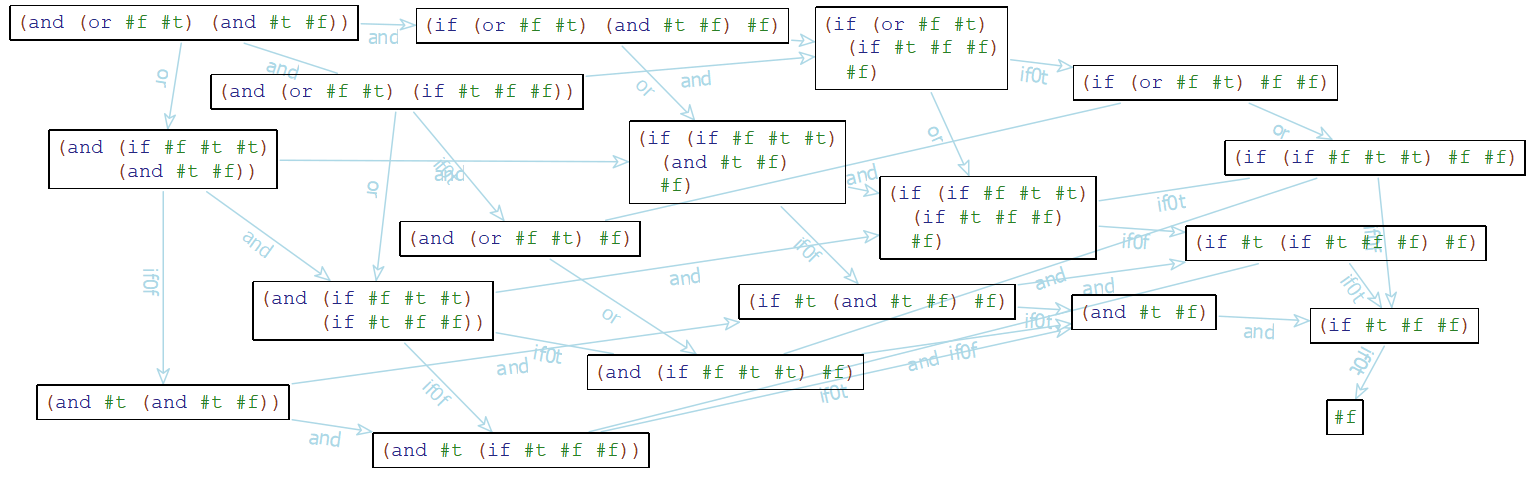
\includegraphics[width=12cm]{images/chapter1/example.png}
	\caption{基本思路}
	\label{fig:base}
\end{figure}

该例子中,对一个结构化(类似S表达式,定义在第二章)的语言,定义其基础语义和规约规则。其中and和or是语法糖,语法糖展开内部语言的if表达式。在没有限制其上下文规则(求值顺序)的前提下,生成了其规约的流程图。我们可以看出,在该图中,既包含了将语法糖展开的规约,也包含了我们期待的$and(\#t,~and(\#t,~\#f))$等等这些中间求值路径。因此我们希望使用基于规约语义的PLT Redex,实现一个轻量级的重组糖,在这个完全图中提取出我们需要的重组糖序列。

在实现过程中,我们发现生成中国完全图并不是必须的,而我们可以在从最初的表达式开始{\bfseries 每次进行单步规约,在一条或多条规约规则中选择我们需要的那条规约规则 }(是本工作的核心算法),且该规则的多次执行保证重组糖的三个基本重要性质。则在这个核心算法迭代执行过程中,会留下一个对应的求值序列,在其中提取出符合输出规则的中间序列,则此序列即为重组糖的输出。


\section{本文主要贡献}
\begin{flushleft}
	1.	我们针对现有重组糖的方法法进行改进,得到新的轻量级重组糖方法。
\end{flushleft}

\begin{itemize}
	\item 我们的方法不需要将所有语法糖都展开就可以得到重组糖序列,而现有方法需要展开后在内部语言执行,并基于match和substitute对可重组的语法糖进行搜索。
	
\end{itemize}

\begin{flushleft}
	2.	我们基于轻量级重组糖算法,用PLT Redex实现了一套工具。
\end{flushleft}
\begin{flushleft}
	3.	基于我们实现的工具,测试得到我们的方法相对于现有重组糖方法,支持更多语法糖特性。
\end{flushleft}

\begin{itemize}
	\item 对递归糖,我们的方法可以很简单的处理。而现有方法只能用letrec处理一下递归绑定。
	\item 对高阶糖,我们的方法也可以很容易处理。而现有方法不能处理。
	\item 对卫生宏,我们的方法处理卫生宏很简单而自然,而现有工作处理卫生宏需要引入新的数据结构以及很多其他处理。
\end{itemize}

\section{全文结构}

我们将在第二章讲述本文工作的一些背景知识及思考路线,第三章讲述工作的算法定义及正确性证明,第四章讲述一些轻量级重组糖的应用,对一些语法糖例子进行讨论评估,第五章对利用PLT Redex的轻量级重组糖工具进行实现上的简单介绍,第六章总结我们的工作,并对一些未来可能的方向进行简单探讨与展望。
